\documentclass[12pt]{elegantbook}

\definecolor{LightGray}{gray}{0.9}
\newcommand{\CN}{BIOS 7300\\[0.5cm] Survival Data Analysis}
\newcommand{\Ti}{Homework 2}
\newcommand{\Pf}{Dr. Tang}
\newcommand{\FN}{Zehao}
\newcommand{\LN}{Wang}
\usepackage[fontsize=14pt]{fontsize}

\usepackage{minted}

\usepackage{enumitem}
\renewcommand{\chaptername}{Homework}
\begin{document}
\begin{titlepage}
    \begin{center}    
    
\includegraphics[width=0.6\textwidth]{Tulane.png}\\[1cm]    
    
    \textsc{\Huge \CN}\\[0.5cm]
    \textsc{\large \Pf}\\[1.0cm]
    
    \textsc{\LARGE \Ti}\\[0.5cm]
    \textsc{\large \LN, \FN}\\
    {Master student in Statistics of Math Dept.}
    
    % Author and supervisor
    
    \vfill
    
    % Bottom of the page
    {\Large \emph{\today}}
    
    \end{center}
\end{titlepage}

\thispagestyle{empty}
\tableofcontents
\setcounter{chapter}{1}
\chapter{}

    % \setcounter{exer}{1}
    \begin{exercise*}[1]
        Here are values of survival time in months from starting of treatment until death or loss of follow-up for 20 cancer patients, with stars indicating right-censored times: 3, 3, 3*, 4*, 5, 5*, 10, 12, 18, 20, 20, 20, 21, 22, 22*, 23 24, 48, 48*, 48*. Group the data into years, and compute the life table estimate of the survivorship and hazard functions by hand, and confirm with software (please include the program and output). 
    \end{exercise*}

    \begin{solution}
        $n'=n_i-c_i/2$; 
        
        Conditional Prob to failure is $d_i/n_i'$;
        
        Prob to survival is $\prod (1-d_i/n_i')$; 

        Prob for Hazard is $\frac{d_i}{(n_i'-d_i/2)T_i}$.
        \begin{table}[h]
        \centering
        \begin{tabular}{lllllll}
        \hline
        Interval & $d_i$ & $c$ & $n_i'$ & Prob to Failure & Survival & Hazard \\ \hline
                $[0,12)$ &  $4$ & $3$  &  $18.5$  &     $0.2162$      &  $1$   &   $0.0202$   \\
                $[12,24)$ &  $8$ & $1$  &  $12.5$  &    $0.64$       &  $0.7838$   &   $0.784$   \\
                $[24,36)$ & $1$  & $0$  &  $4$  &     $0.25$      &  $0.2822$   &    $0.0238$  \\
                $[36,48)$ & $0$  & $0$  &  $3$  &    $0$       &  $0.2116$   &   $0$   \\
                $[48,\cdot)$ & $1$  &  $2$ &  $2$  &     $0.5$      &   $0.2116$  &   $\cdot$   \\ \hline
        \end{tabular}
        \end{table}

        The Results in SAS: 
        \begin{minted}[frame=lines,
            framesep=2mm,
            baselinestretch=1.2,
            bgcolor=LightGray,
            fontsize=\footnotesize,
            linenos]{sas}
            DATA HW1_1;
            INUPT id time is_censoring;
            DATALINES;
            1 3 0
            2 3 0
            3 3 1
            4 4 1
            5 5 0
            6 5 1
            7 10 0
            8 12 0
            9 18 0
            10 20 0
            11 20 0
            12 20 0
            13 21 0
            14 22 0
            15 22 1
            16 23 0
            17 24 0
            18 48 0
            19 48 1
            20 48 1
            ;
            RUN;
            PROC LIFETEST 
            DATA=HW1_1 
            METHOD=lt 
            INTERVALS=(12 TO 48 BY 12);
            TIME time*is_censoring(1);
            RUN;
        \end{minted}
        \begin{figure}[h]
        \centering
        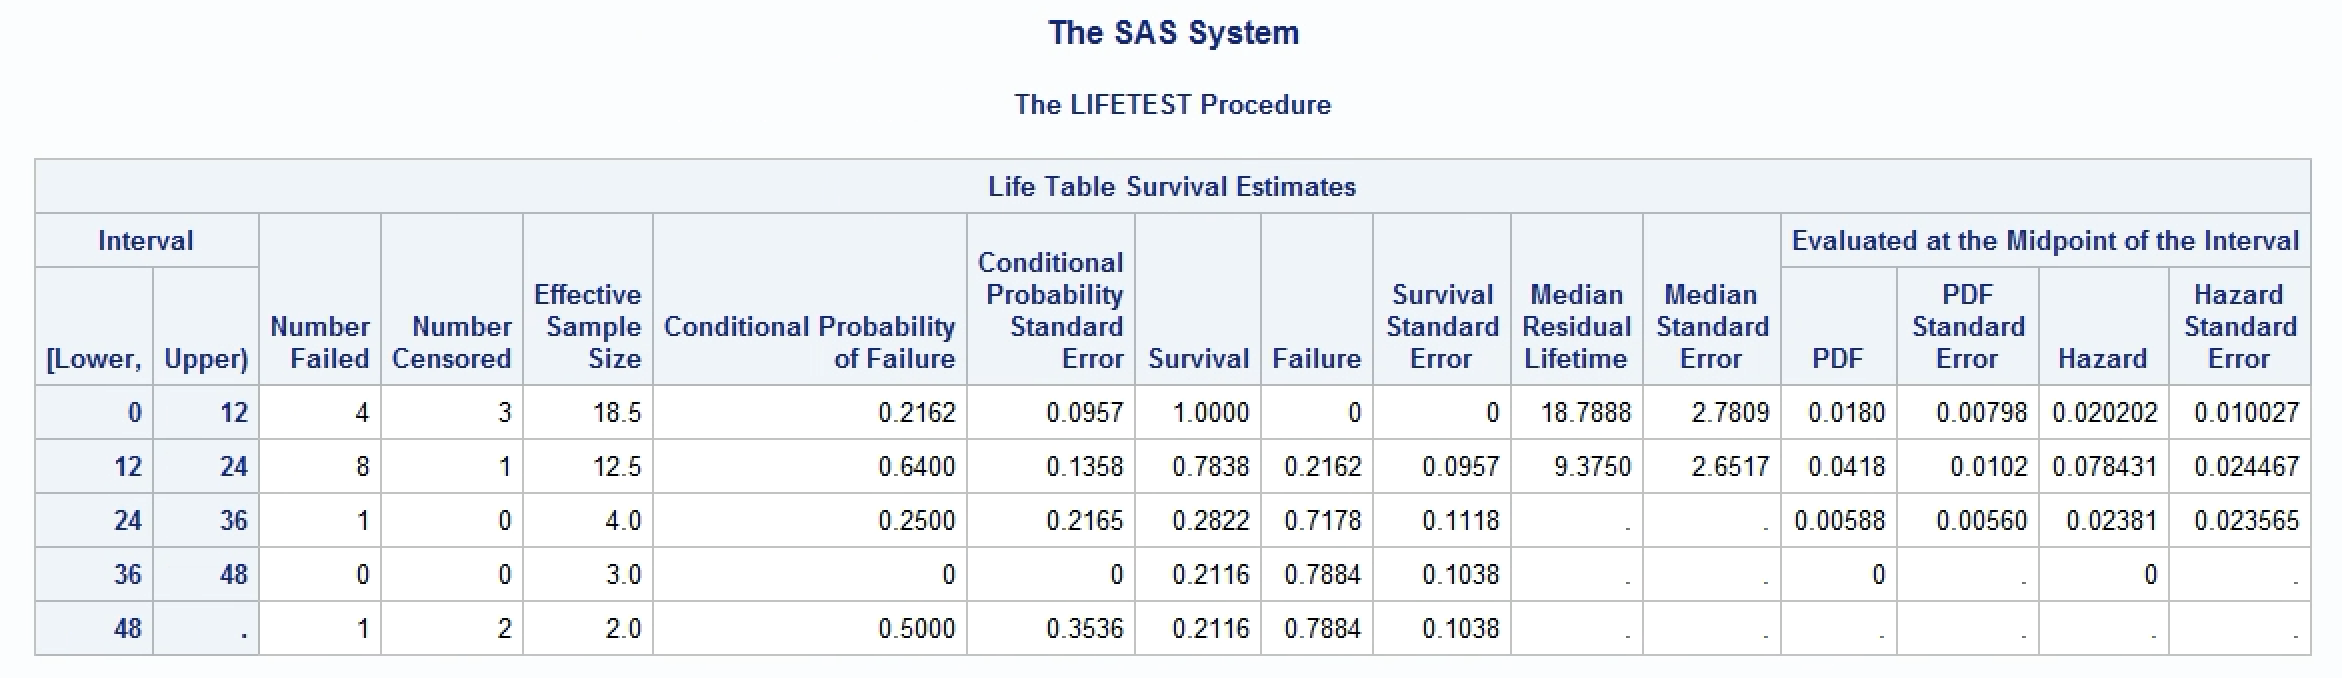
\includegraphics[width=\textwidth]{HW1_1.png}
        \end{figure}
    \end{solution}

    \begin{exercise*}[2]
        Using the data in Problem 1, manually estimate the following functions up to and including time 12: 
        \begin{enumerate}[(a)]
            \item The Kaplan-Meier estimate of the survivorship function.
            \item The variances of the Kaplan-Meier estimate you obtained for the survivorship function in Part (a). 
            \item The hazard function. 
        \end{enumerate}
    \end{exercise*}

    \begin{solution}
        include 12 but not include 18. 

        $\hat{S}(t)=\prod_{t_{(i)}<t}\frac{n_i-d_i}{n_i}$

        $Var(\hat{S}(t))=\hat{S}(t)^2\sum_{t_{(i)}<t}\frac{d_i}{n_i(n_i-d_i)}$

        $h(t)=\frac{d_i}{n_i(t_{i+1}-t_i)},\quad t_i<t<t_{i+1}$
        \begin{table}[H]
        \centering
        \begin{tabular}{llllllll}
        \hline
        Interval & $n_i$ & $d_i$ & $c_i$ & $1-d_i/n_i$ & $\hat{S}(t)$ & Var & $h(t)$ \\ \hline
                $[0,3)$ &  $20$ & $0$  & $0$ & $1$  &     $1$      &   $0$   & $0$  \\
                $[3,4)$ &  $20$ & $2$  &  $1$  &    $0.9$       &  $0.9$   &   $0.0045$ & $0.1$ \\
                $[4,5)$ & $17$  & $0$  &  $1$  &     $1$      &  $0.9$   &    $0.0045$ & $0$ \\
                $[5,10)$ & $16$  & $1$  &  $1$  &    $0.9375$       &  $0.8438$   &   $0.0069$  & $0.0125$ \\
                $[10,12)$ & $14$  &  $1$ &  $0$  &     $0.9286$      &   $0.7835$  &   $0.0093$ & $0.0357$ \\ 
                $[12,18)$ & $13$  &  $1$ &  $0$  &     $0.9231$      &   $0.7232$  &   $0.0113$  & $0.0128$ \\ \hline
        \end{tabular}
        \end{table}
    \end{solution}
    
    \begin{exercise*}[3]
        The file ``Survival of liver transplant recipients.dat'' contains data from a liver transplant study. The survival time (in days) is from the liver transplant to graft failure. The variable “time” records the failure time or censoring time, and the variable ``status'' is the indicator for failure ($=1$ if failure observed and $=0$ is censored). Use software to estimate the survival function and pointwise $95\%$ confidence interval. 
    \end{exercise*}

    \begin{solution}
        \begin{minted}[frame=lines,
            framesep=2mm,
            baselinestretch=1.2,
            bgcolor=LightGray,
            fontsize=\footnotesize,
            linenos]{sas}
            DATA HW1_2;
            INFILE "Z:\Desktop\HW1_2.dat" FIRSTOBS=2;
            INPUT 
                patient 1-5 
                age 6-12 
                gender 13-18 
                disease 19-25
                time 26-34
                status 35-41
                cof 42-50;
            RUN;
            PROC LIFETEST 
                DATA=HW1_2 
                METHOD=km 
                PLOTS=s(cl);
            TIME time*status(0);
            SURVIVAL OUT=ci 
                CONFTYPE=loglog 
                STDERR;
            RUN;
            PROC PRINT DATA=ci;
            RUN;
        \end{minted}
        \begin{figure}[H]
            \centering
            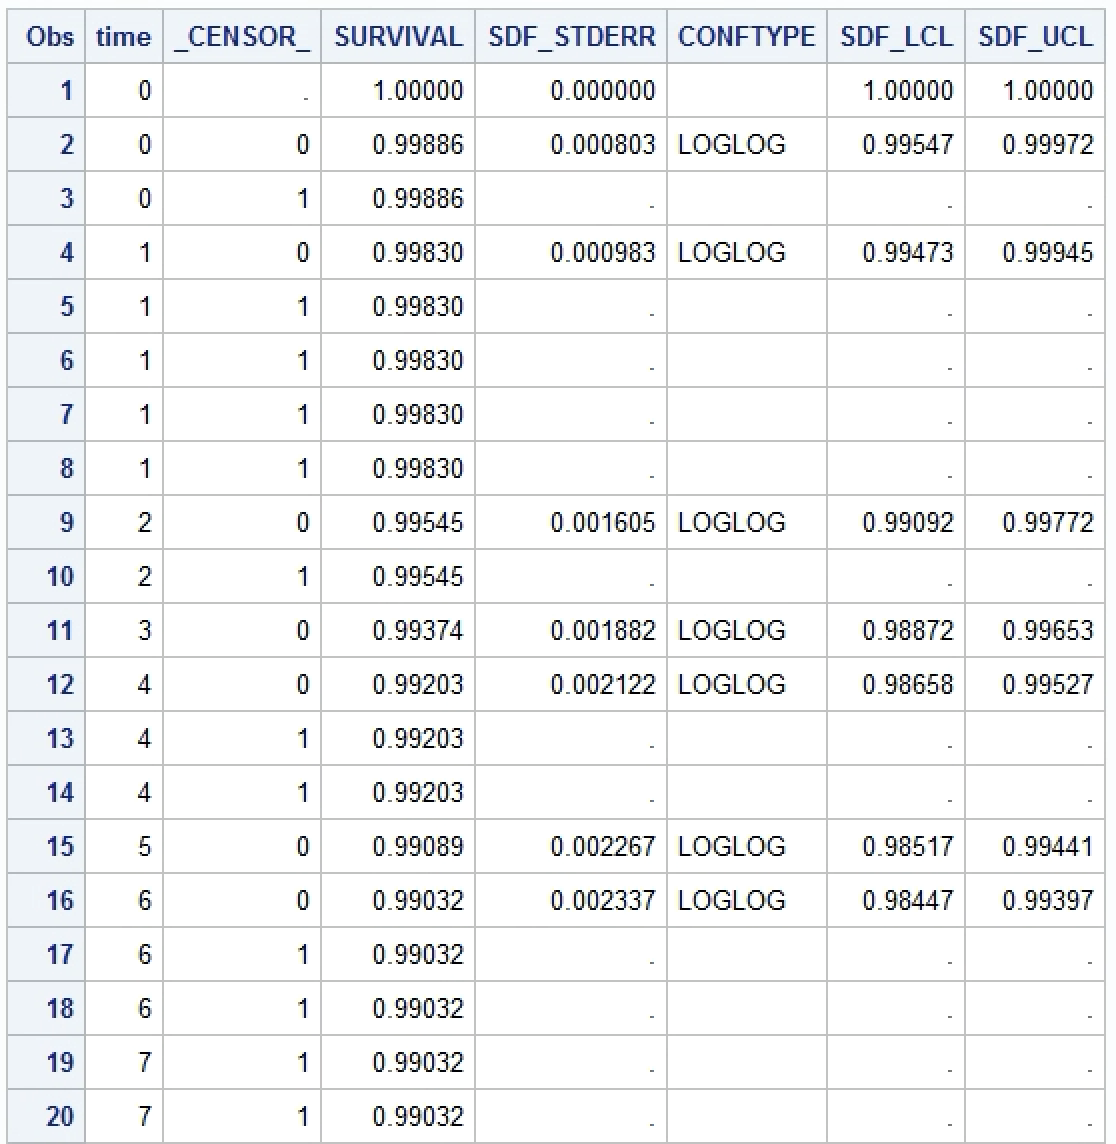
\includegraphics[width=\textwidth]{HW1_3.png}
        \end{figure}
    \end{solution}
    
    \begin{exercise*}[4]
        The following table contains the KM estimate of the survival function ($S$) and its point-wise confidence intervals (LCL=lower limit and UCL=upper limit), where $c$ is the censoring indicator (0 means not censored, and 1 means censored). Based on the table, find the following quantities. If any of these quantities are undefined, explain. 
        \begin{enumerate}[(a)]
            \item The median survival time, and the $95\%$ confidence interval for the median.
            \item The first and third quartiles, and the $95\%$ confidence intervals for these quartiles.
            \item The SIQR. 
        \end{enumerate}
        \begin{figure}[H]
            \centering
            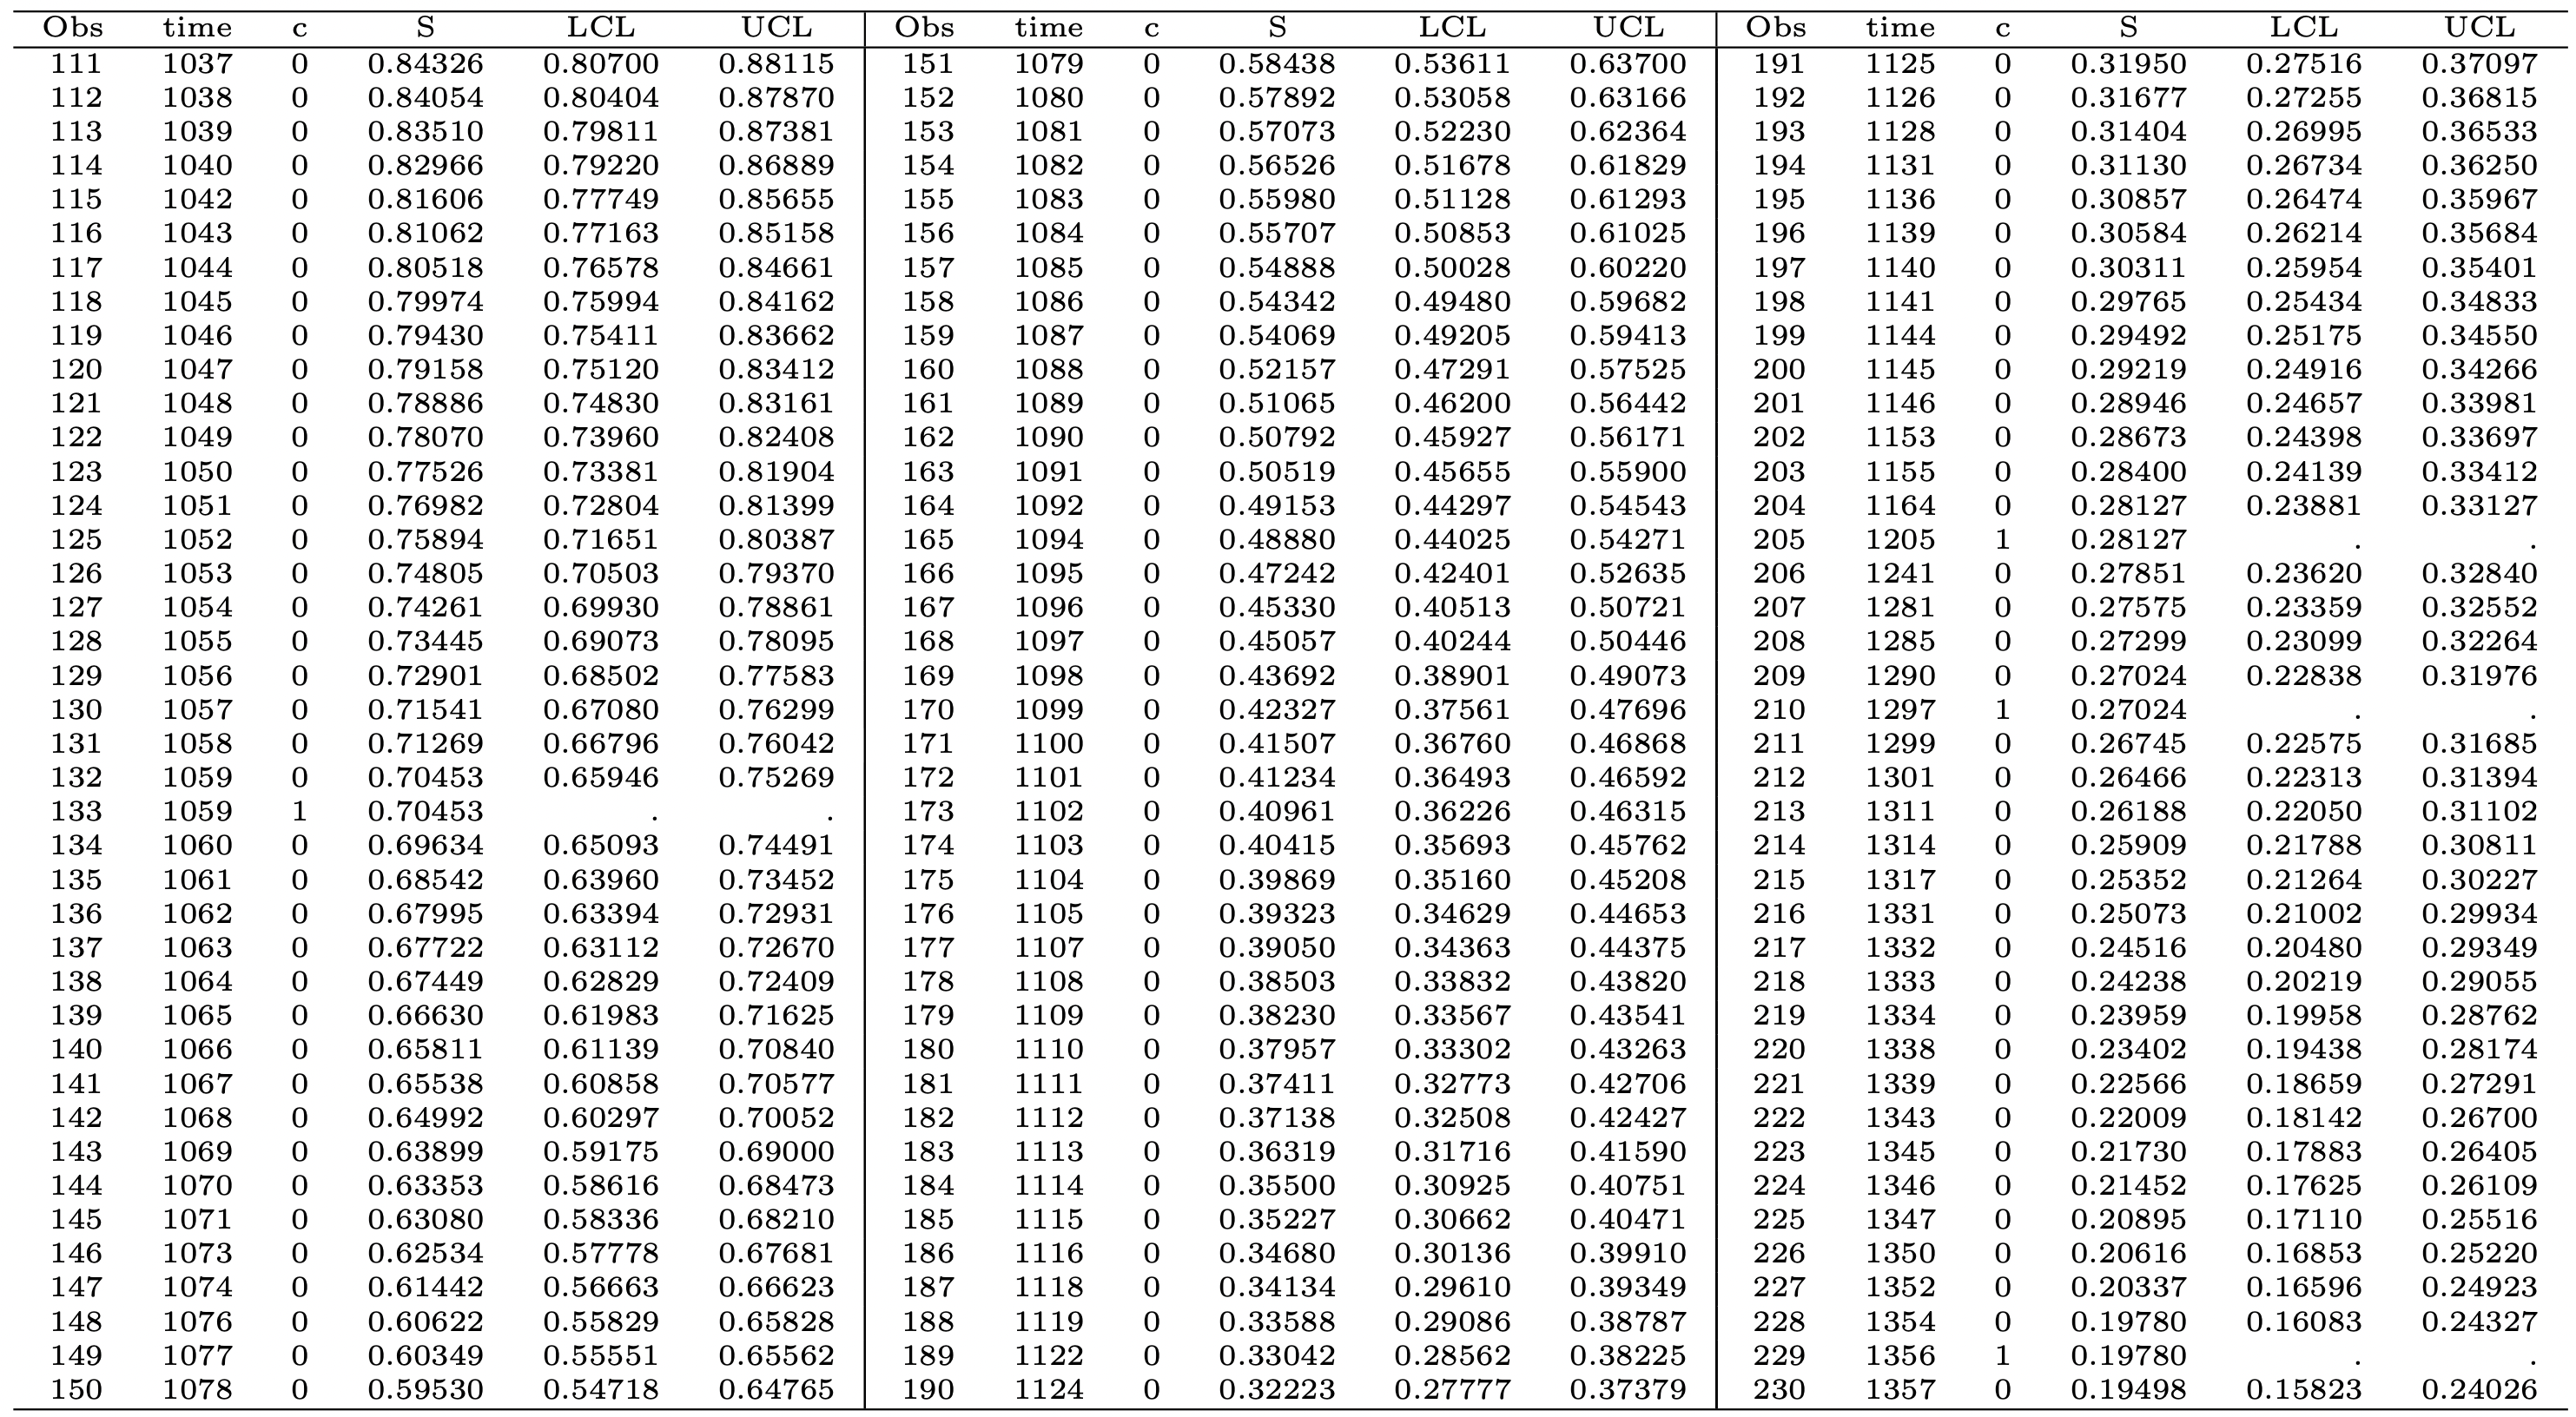
\includegraphics[width=\textwidth]{HW1_4.png}
        \end{figure}
    \end{exercise*}
    \begin{solution}
        \begin{enumerate}[(a)]
            \item Median survival time is: $t=\min\{t:S(t)\leq0.5\}=1092$. With this same condition on LCL and UCL, we can get the $95\%$ confidence interval for the median is $[t_{LCL},t_{UCL}]=[1086,1098]$. 
            \item First quartile is: $t=\min\{t:S(t)\leq0.75\}=1053$. And the $95\%$ confidence interval for the first quartile is $[t_{LCL},t_{UCL}]=[1053,1060]$. 
            
            Third quartile is: $t=\min\{t:S(t)\leq0.25\}=1332$. The $95\%$ confidence interval for the third quartile is $[t_{LCL},t_{UCL}]=[1145,1352]$. 
            \item \[SIQR=(t_{0.75}-t_{0.25})/2=139.5. \]
        \end{enumerate}
    \end{solution}
\end{document}